\graphicspath{{Chapters/Chapter_background/}}

\chapter{Background}
\label{ch:background}

%Given the LAPD parameters in this study (tables ref), the collision frequencies are sufficiently high such that the mirror is in the gas-dynamic regime: losses out of the mirror throat are governed by collisions. The mirror length must exceed the scattering into the loss cone\cite{Ivanov_2013}:
%\begin{equation}
%    L > \lambda_{ii} \cdot \ln{R} / R
%\end{equation}
%These collisions populate the loss cone and maintain a Maxwellian distribution, eliminating the possibility of loss-cone-driven instabilities like the AIC or DCLC instabilities that have been observed in hotter devices
%
%\section{Instabilities in mirrors}
%\subsection{Interchange}
%
%At low $\beta$, as we are in the LAPD, the flute instability is a purely electrostatic perturbation. The growth rate of interchange is approximately \cite{Ryutov_2011}
%\begin{equation}
%    \Gamma_0 = \frac{c_s}{\sqrt{L_M L}}
%\end{equation}
%where $L_M$ is the length of the mirror section measured where the curvature flattens out on either end of the cell and $L$ is the total length of the plasma. The distinction between the length of the mirror and the length of the plasma is important because the instability is driven by the pressure of the plasma where the magnetic field has curvature, but the inertia of the plasma comes from it's total volume. Just for some numbers, assuming $c_s \approx 10$ km/s, $L_M \approx 7$ m, and $L \approx 17$ m, one expects a growth rate of $\Gamma_0 \approx 1.2$ kHz.
%
%The interchange instability occurs when the density gradient and magnetic curvature, when integrated along the field line, point in the same direction. 
%Stabilization by finite Larmor radius (FLR) effects \cite{Post_1987}:
%\begin{equation}
%    \frac{a_i}{r_p} > \frac{m^{1/2}}{m-1} \frac{r_p}{L}
%\end{equation}
%Our ions are so cold that FLR effects only become significant when $m \gtrsim 300$
%
%Line-tying and vortex stabilization 
%
%\subsection{Alfvén ion cyclotron (AIC)}
%\subsection{Drift cyclotron loss cone (DCLC)}

\section{The Large Plasma Device at UCLA}

The Large Plasma Device (LAPD)\cite{gekelman_upgraded_2016,qian_design_2023} is a 26 meter long linear plasma device located Basic Plasma Science Facility (BaPSF) at the University of California, Los Angeles. This device is built for basic plasma science and can create quiescent, long-lived (read: longer than the timescales of interest) plasmas. The LAPD produces up to 18 m long, 1 m diameter plasmas. A cartoon of the LAPD and the canonical coordinate system can be seen in fig. \ref{fig:lapd-pics}.

\begin{figure}
	\centering
	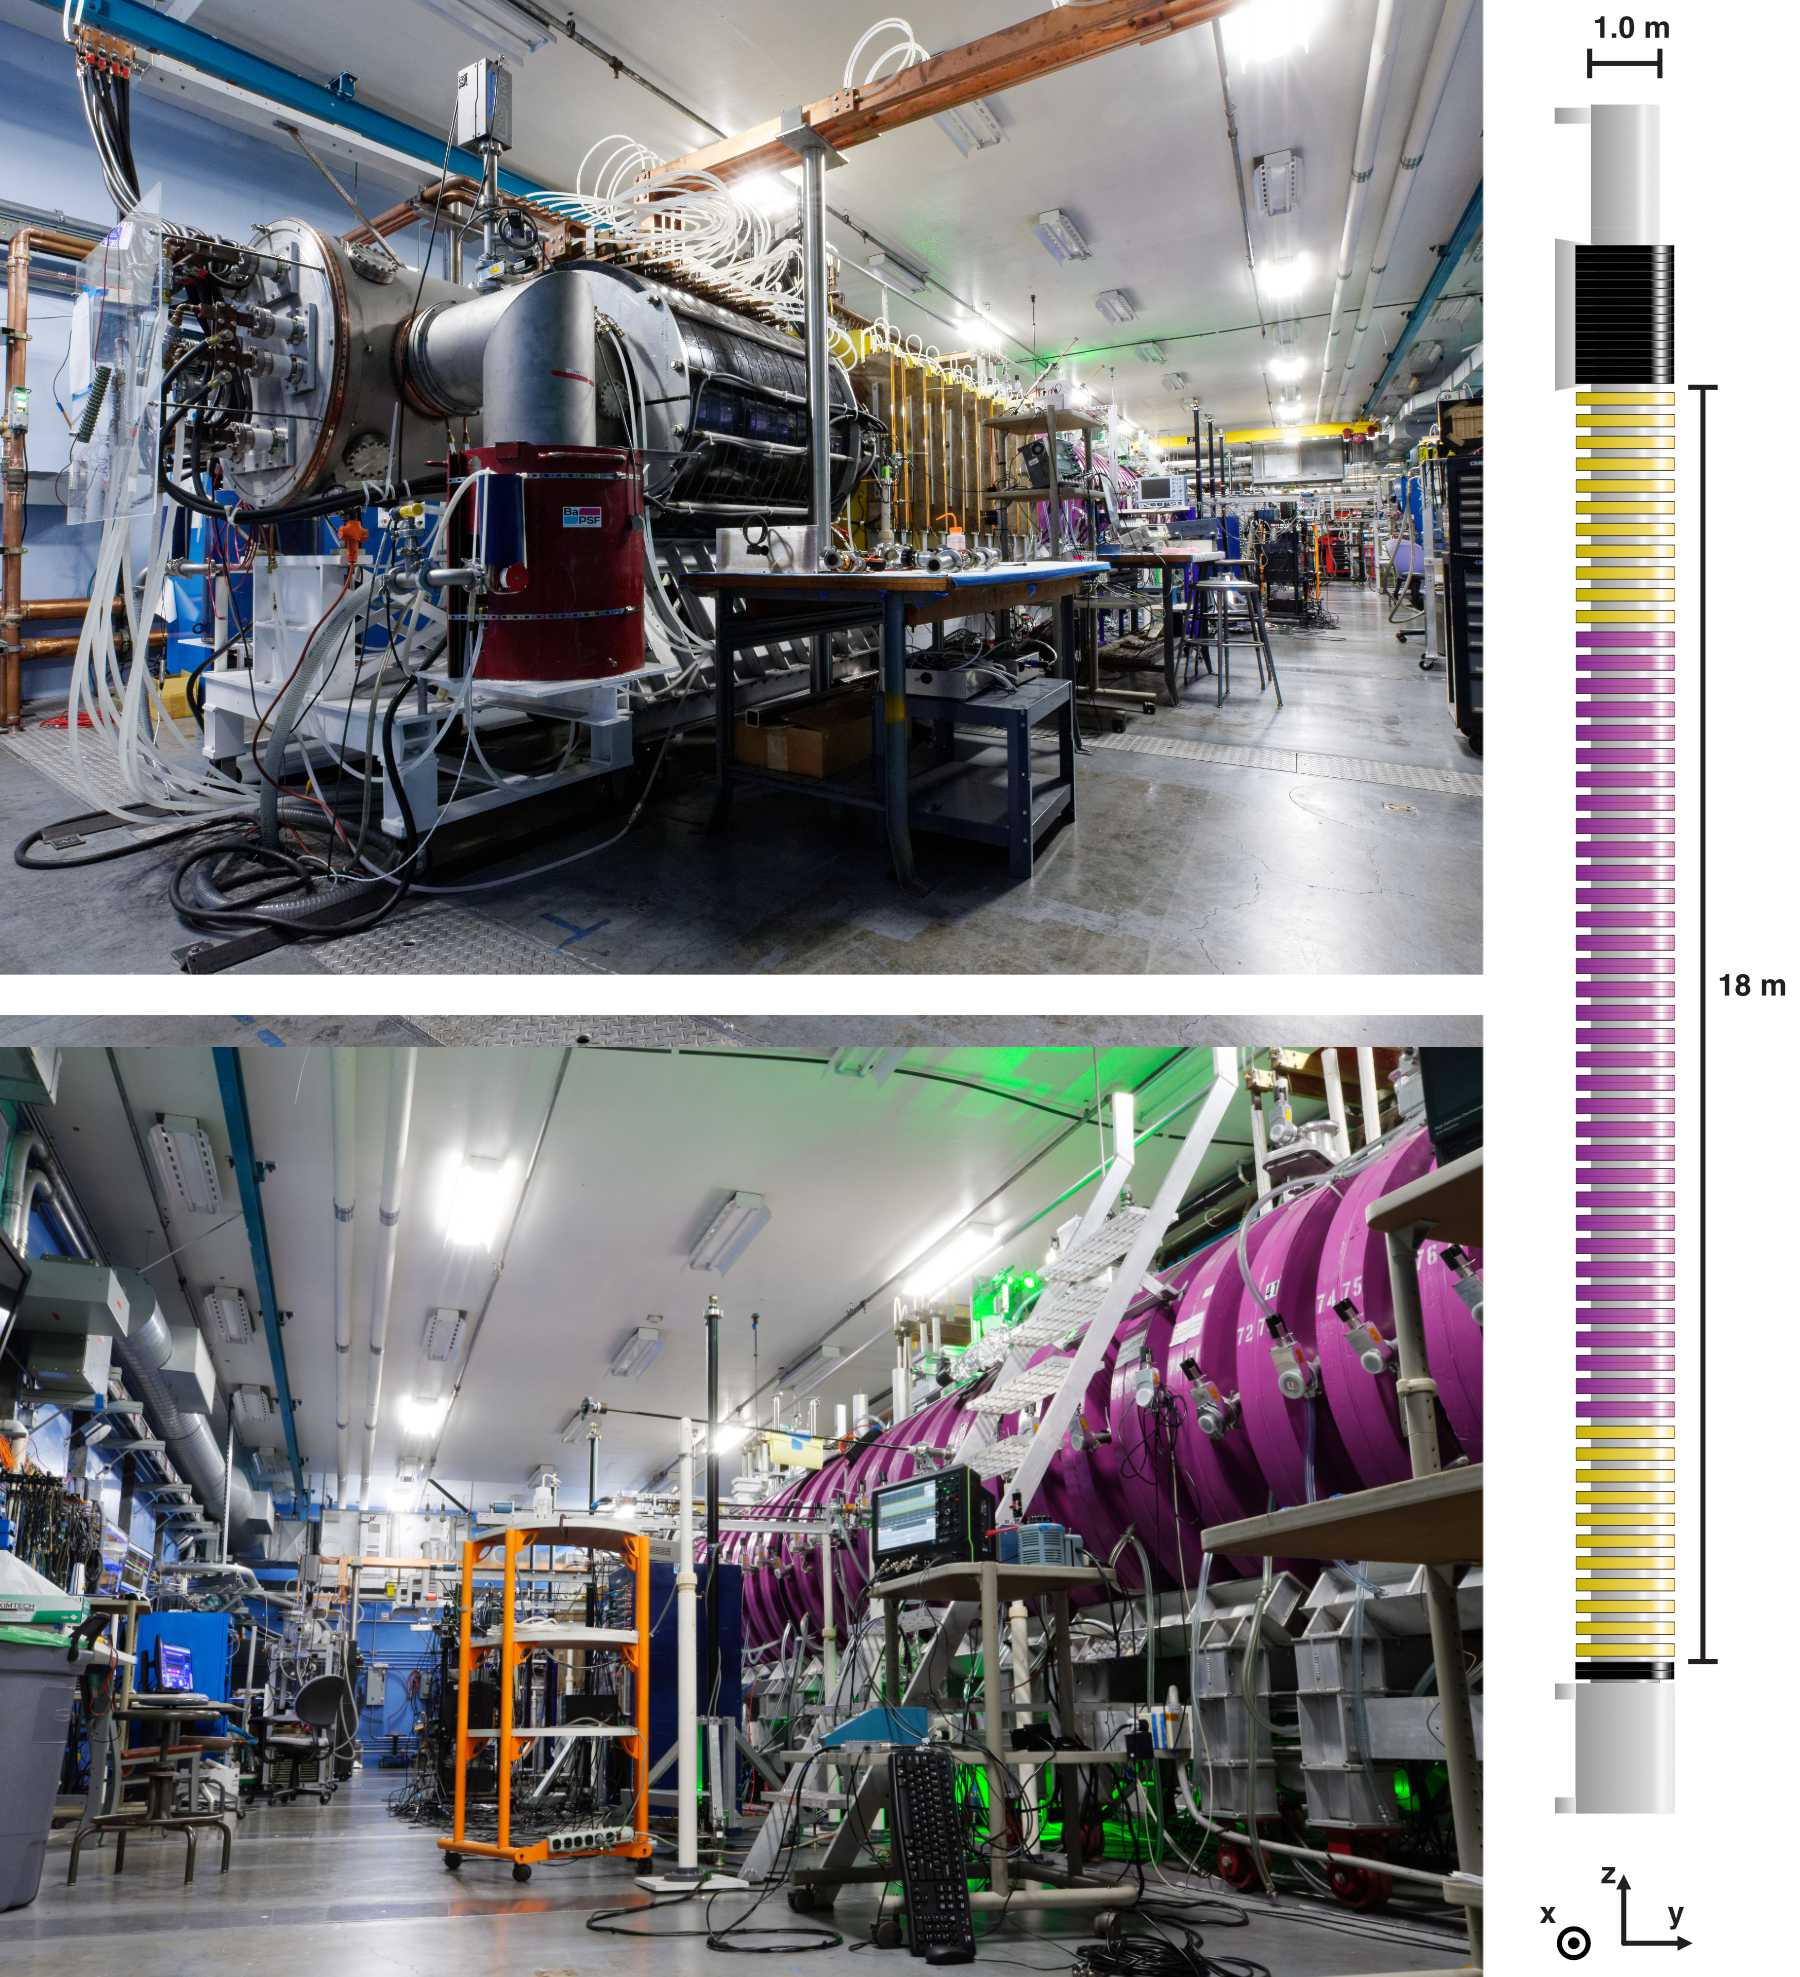
\includegraphics[width=400pt]{figures/lapd_pics.jpg}
	\caption[Pictures of the LAPD]{\label{fig:lapd-pics}Top: picture from the LAPD taken from the south end of the device, next to the cathode and anode region. Bottom: picture taken in the middle section closer to the north end. Right: cartoon of the LAPD with the coordinate system used.}
\end{figure}

\subsection{Plasma source}

Typically, plasmas are produced using a hot cathode and anode at the south end of the device. This cathode was originally barium oxide (BaO)-plated nickel \cite{gekelman_upgraded_2016}, but was recently upgrade to a segmented lanthanum hexaboride (LaB$_6$) source \cite{qian_design_2023}. The BaO cathode was $72$ cm in diameter which mapped to 60 cm in a flat field magnetic field configuration. A $72$ cm diameter, 50\% transparent molybdenum anode was used to accelerate electrons from the cathode down the length of the machine. This BaO source could reach densities of $4 \times 10^{12}$ cm$^{-3}$ and up to 8 eV. The LaB$_6$ cathode is 35 cm across and electrons are accelerated through a 64.4 cm diameter, 66\% transparent molybdenum anode. The LaB$_6$ cathode can form hotter, denser plasmas with densities up to $3 \times 10^{13}$ cm$^{-3}$ and temperatures up to 20 eV, though typical operation yields temperatures around 5 eV, and is also more robust to accidental atmospheric exposure. The LaB$_6$ cathode is heated to $\approx$ 1700 $^\circ$C using a $\approx$2 kA heater. Both of these cathodes were used in the work presented here. An insertable, smaller (20 cm diameter) LaB$_6$ source also exists at the north end of the machine but is not used in this work. An interior shot of the LAPD can be seen in fig. \ref{fig:lapd-inside}.

\begin{figure}
	\centering
	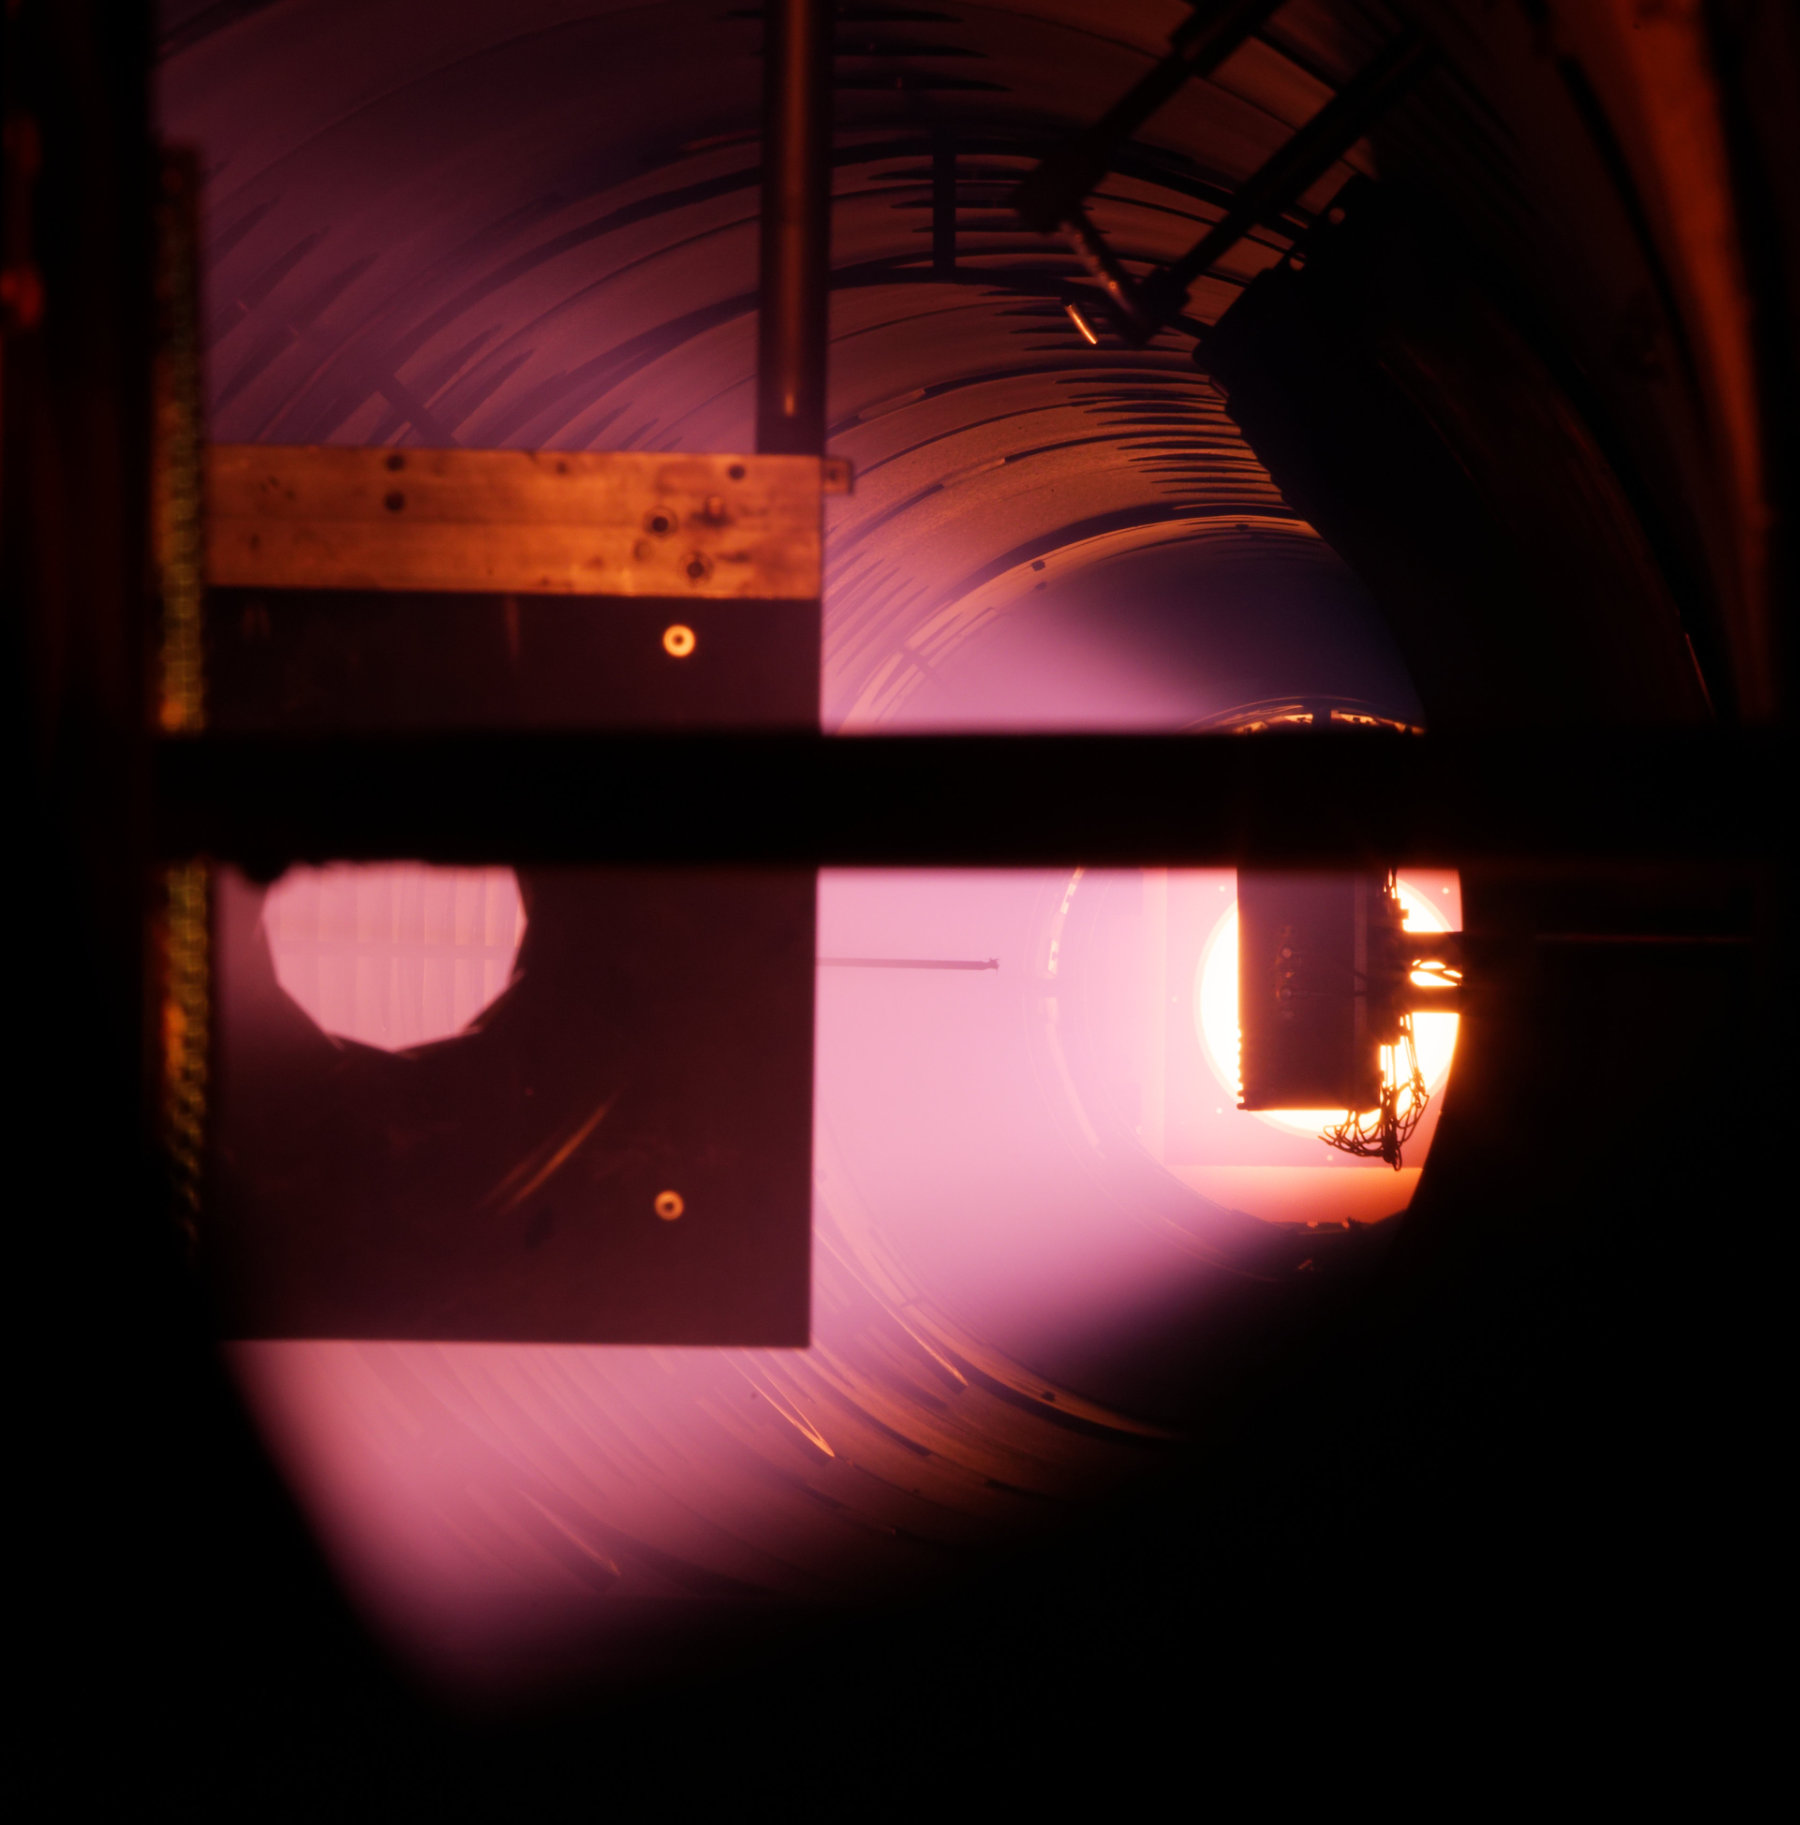
\includegraphics[width=350pt]{figures/lapd_inside.jpg}
	\caption[Picture of LAPD interior]{\label{fig:lapd-inside}The interior of the LAPD taken during a discharge from the end of the machine. The hot LaB$_6$ cathode can be seen at the far end. Inside the plasma chamber are, from left to right, a carbon iris (used in Josh Larson's experiments) for controlling the width of the plasma from the smaller north-end source, an electric dipole probe, and the traveling wave antenna. The pink glow is the plasma formed by the far, main LaB$_6$ source. This picture was included for no other reason other than it's a banger.}
\end{figure}


The voltage applied across the cathode and anode is supplied by a 4.2 Farad capacitor bank switched by group of IGBTs. The discharge voltage is configurable up to 180V before triggering the over-voltage protection, though the capacitors are rated up to 200V. Current through the cathode can exceed 10 kA. Discharges can last as long as 70 ms, though a typical duration is around 15-20 ms. Discharge duration, power, and repetition rate are governed by the size of the capacitor bank and the charging power supply. The discharge repetition rate is configurable between 0.1 and 1 Hz.

\subsection{Magnetic field}
The LAPD has 13 independently-configurable magnet power supplies to shape the geometry of the axial magnetic field. Two of the supplies control the source region field, one controls the north end field where the smaller LaB$_6$ source resides, and the remaining 10 supplies control the field of the main plasma column. The source field can reach up to 8 kG and the main plasma column field up to 1.6 kG. A 1 kG field leads to an ion gyroradius of 2 mm at 1 eV, and a electron gyroradius of 50 $\mu$m at 5 eV, so these plasmas are highly magnetized. The source field is set manually on the power supplies themselves, but the middle 10 fields can be programmed on the LabView housekeeping system.

\subsection{Gas fueling}
There are two main ways of providing the neutral gas necessary for producing plasmas: the static fill system and gas puffing. The static fill system utilizes mass flow controllers to fill the chamber to the desired pressure, usually between $10^{-5}$ and $5 \times 10^{-4}$ Torr. The LAPD can be filled with a variety of (nonreactive) gasses, helium being the most common, followed by hydrogen and argon. The gas puff system utilizes piezo valves to puff gas into the chamber halfway between the cathode and anode. Gas puff duration and valve voltage can be set which influence the total amount of gas puffed and thus plasma density. Plasma  breakdown using gas puffing is very reliable. Without fueling the LAPD has a base pressure of 5 $\times 10^{-7}$ Torr. The pressure is constantly monitored by the housekeeping system. 

\section{Data acquisition}

Probes can sample virtually any point in this plasma through unique ball valves placed every $\approx$32 cm along the length of the device, enabling the collection of time series data with high spatial resolution. Four probe drives can simultaneously be used to move probes in the x-y plane. An x-y-z probe drive is also available for collecting volumetric data. There are also 3 permanently attached probe drives mounted 45$^\circ$ up from the -x axis, on which, at the time of this writing, are mounted Langmuir probes. These drives have a limited motion compared to the standard x-y probe drives used during dataruns and the signals are digitized on 8-bit oscilloscopes. Typically many shots are taken at one position to obtain good sample statistics.

Primarily, probe data acquisition is handled through the main data acquisition system, simply referred to as the ``DAQ''. The DAQ consists of SIS 3302 digitizers (theoretically 32 channels total) capable of sampling signals between $\pm 2.5$ V at 100 MHz at 16 bits. Typically sample averages are taken (16 samples for my data) to reduce data transfer and file size. The DAQ is set up through a LabView-based control system. 

This LabView system manages ``dataruns'' which are a series of discharges with a particular LAPD configuration (including the DAQ, probe motion control, and other device configurations such as function generators). Another LabView system controls the probe movements. All these devices are enabled and commands in a particular order via the run sequencer. 

Another LabView system manages the machine state information (MSI). This system collects information on the discharge (current, voltage), auxiliary diagnostic signals (and it used to record interferometer), gas total pressure and RGA pressures. The time series diagnostics are read by a National Instruments PCIe-6346 data acquisition card which samples with 16 bits over 8 analog inputs at 500 kS/s per input. The MSI also collects information on the state of the magnetic field and cathode heater from the housekeeping system. An auxiliary python system can also be used collate diagnostics from multiple sources, including the machine state information.

\section{Diagnostics}

LAPD can field many different diagnostics and other equipment through the ball-valve ports as well as much larger box-shaped ports.
Probe diagnostics typically go through an isolation amplifier before heading into the DAQ, along with attenuators so the signals fit the DAQ range

\subsection{Langmuir probes: $I_\text{sat}$, sweeps, triple probes}

Langmuir probes (LPs) are a workhorse of diagnostics in low temperature plasmas, such as the LAPD, and are also used at the (lower temperature) edge of fusion devices. These probes can be used to measure density, temperature, and potential of the plasma. LPs are essentially a conductive tip (typically tungsten in our case) inserted into the plasma. Three different types of these LPs can be seen in fig. \ref{fig:langmuir_tips}. 

\begin{figure}
	\centering
	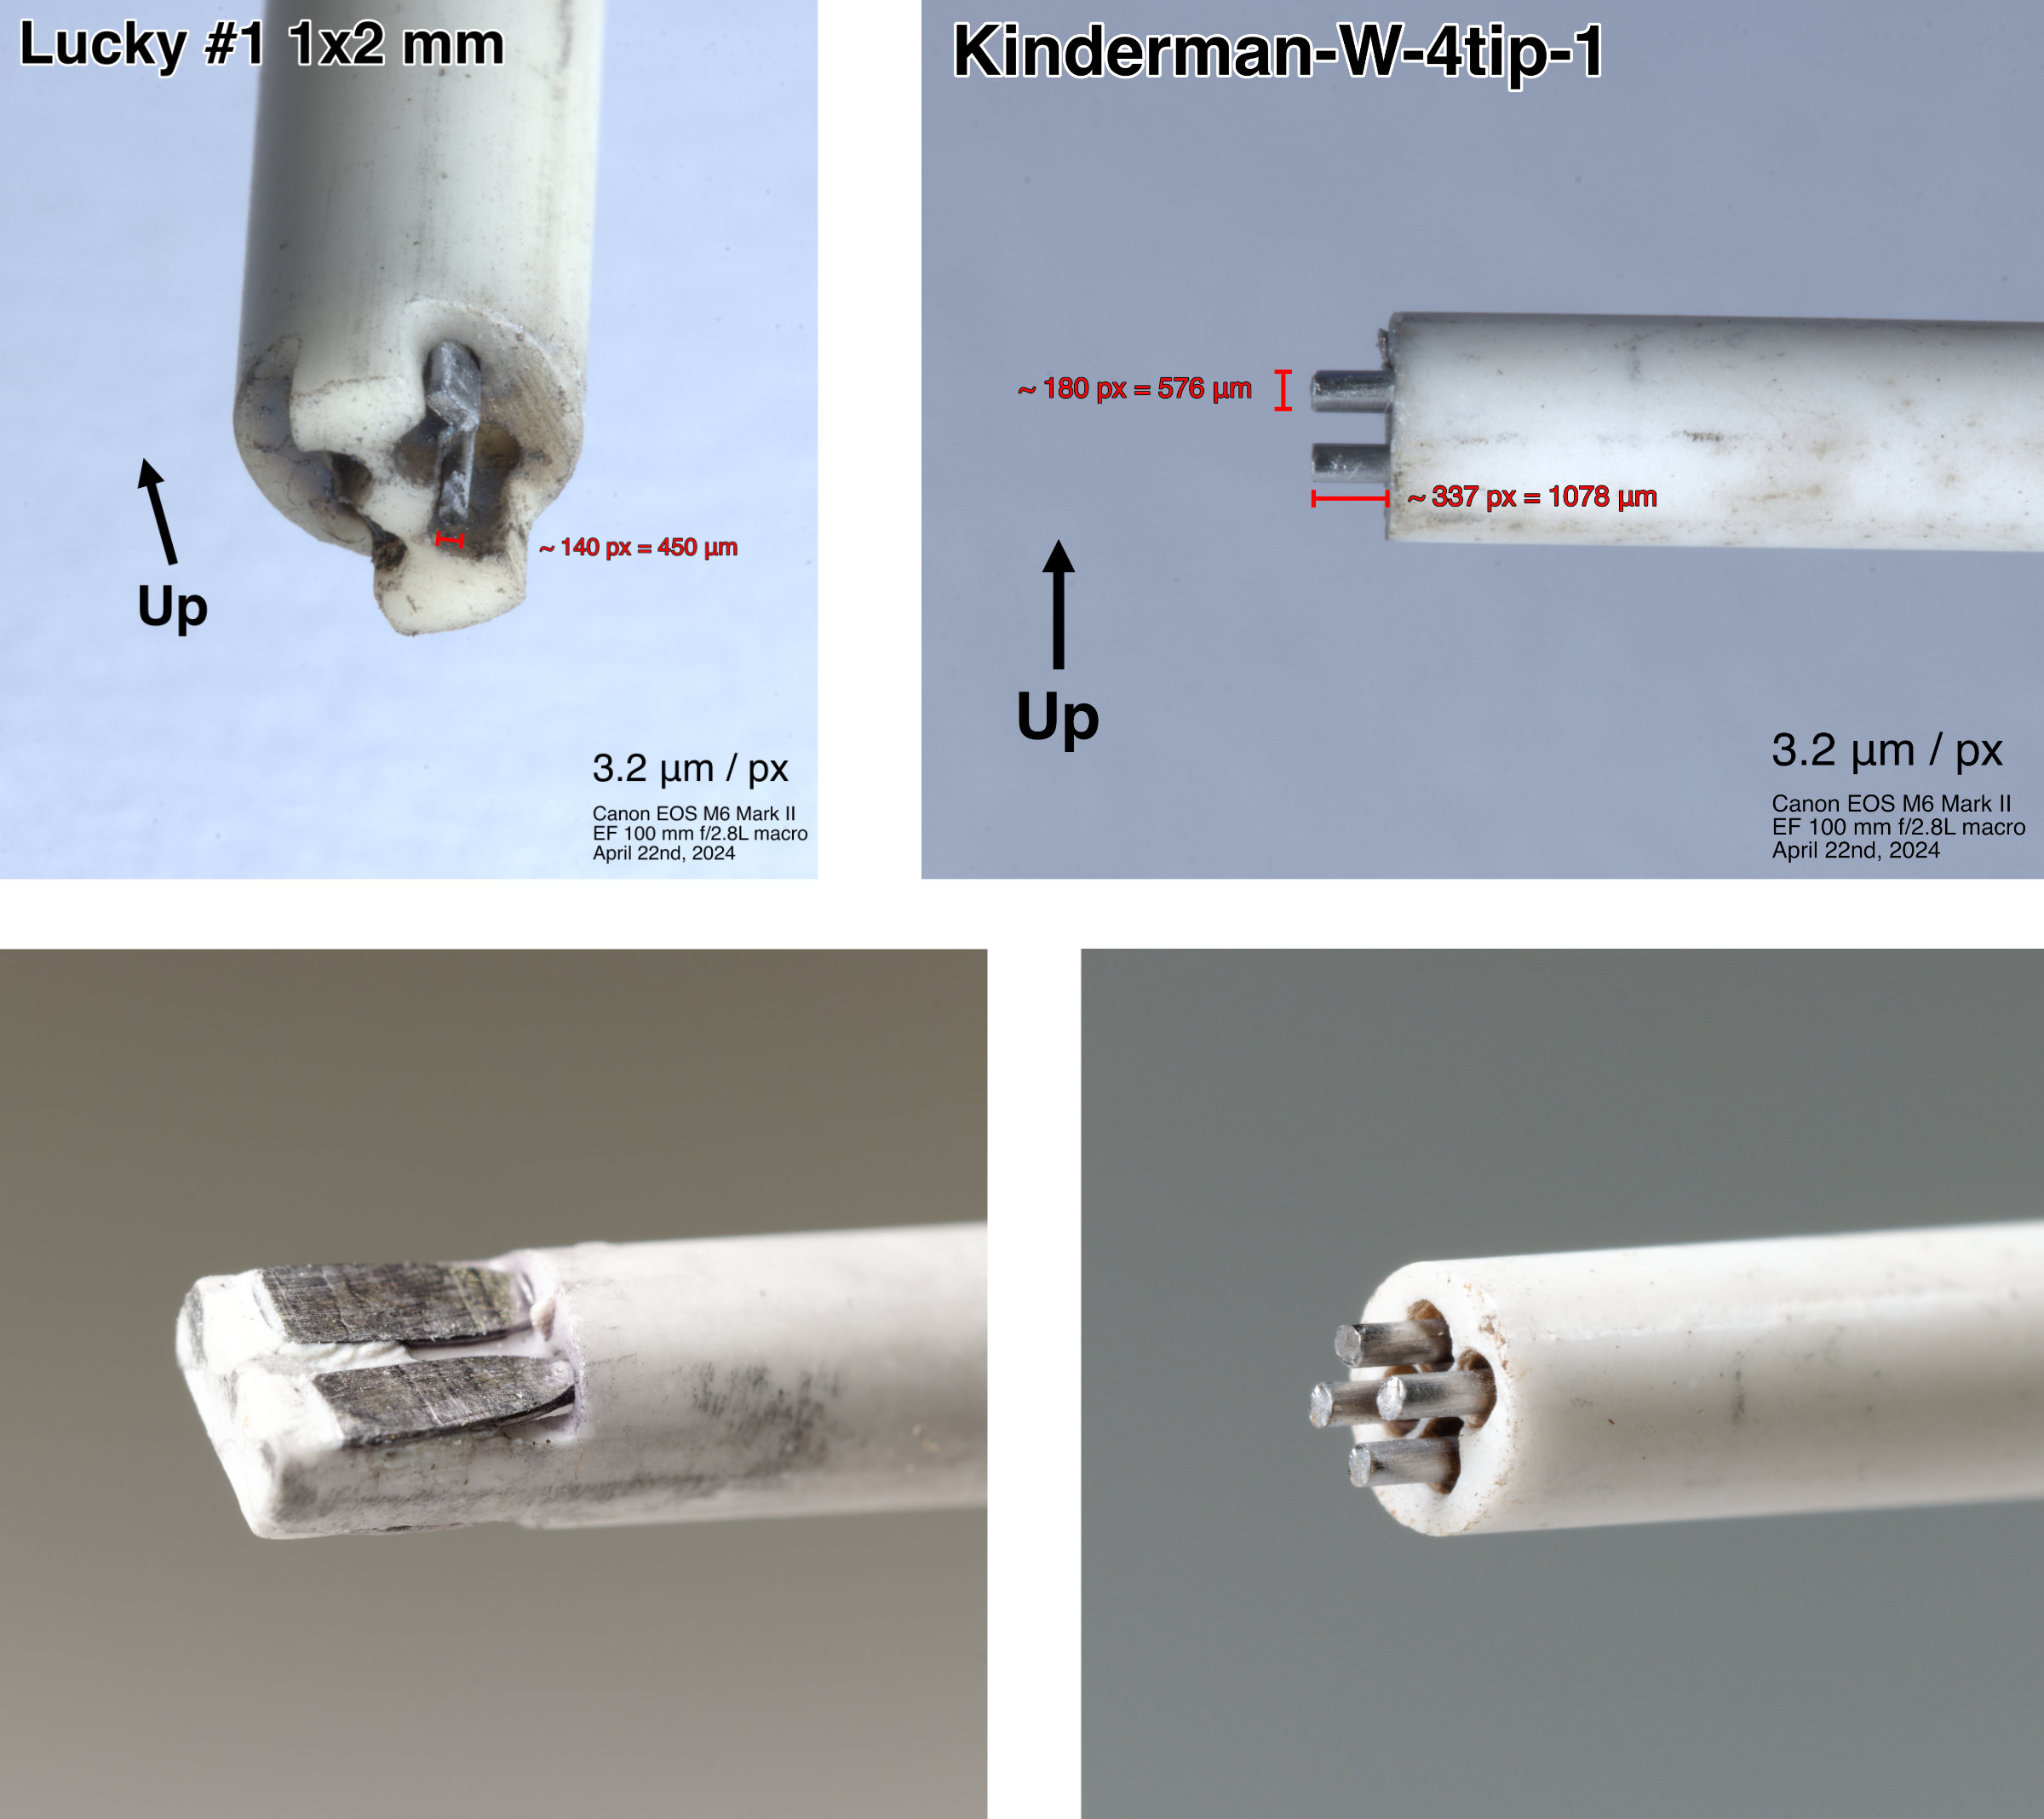
\includegraphics[width=\textwidth]{figures/langmuir_pics.jpg}
	\caption[Images of Langmuir probes used in the LAPD]{\label{fig:langmuir_tips}Three different types of Langmuir probes used in the LAPD: flat protruding tips (top left), flat, flush tips (bottom left), and cylindrical tips (right). Probe areas are often not as advertised based on measurements using a camera and macro lens.}
\end{figure}

The LP can be biased to measure different portions of the current-voltage relationship. Common biasing schemes are: applying a strong negative bias, sweeping the bias along a set range, free-floating the tip, and biasing another tip via the ion saturation current  from another tip. The I-V relationship of a LP and the quantities deduced from it can be seen in fig. \ref{fig:langmuir_sweep} which will be detailed below.

\begin{figure}
	\centering
	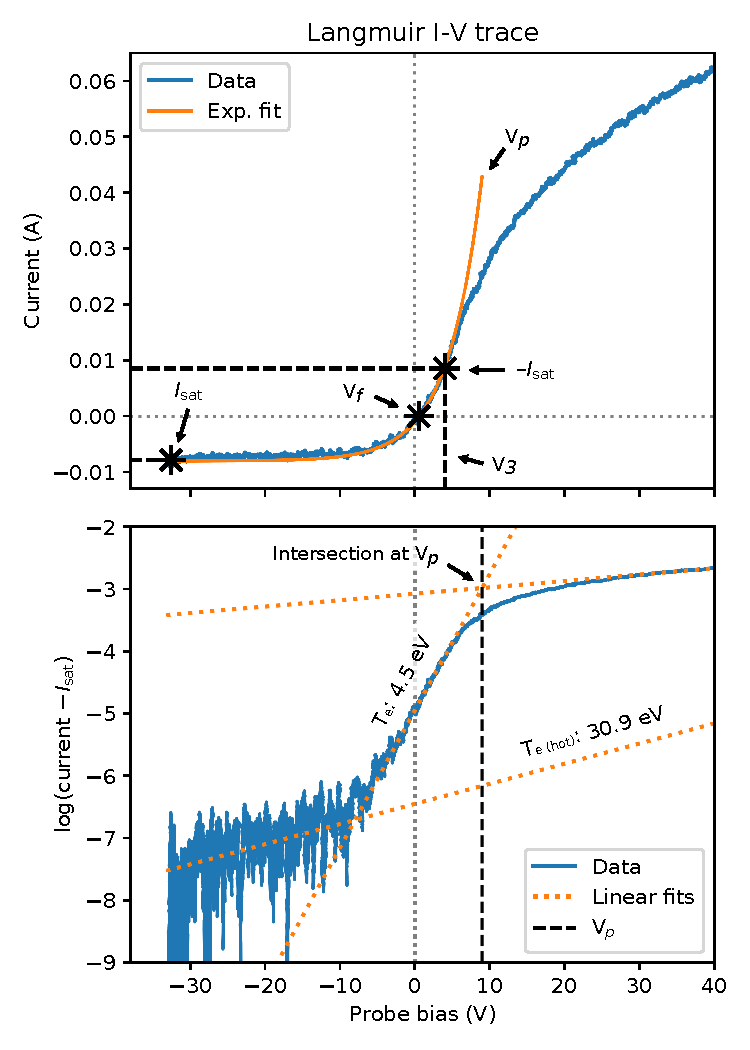
\includegraphics[height=0.8\textheight]{figures/example_sweep_analysis.pdf}
	\caption[Typical Langmuir probe I-V curve]{\label{fig:langmuir_sweep}Typical Langmuir probe I-V curve on top, with a logarithmically-scaled version on the bottom (with $I_\text{sat}$ subtracted). The log-scaled version is typically used for fitting the temperature(s). Useful points on the curve are labeled.}
\end{figure}

\subsubsection{Ion saturation current ($I_\text{sat}$)}
When the LP tip is biased negatively, the probe tips rejects all electrons and only collect ions, and is thus called the ion saturation current. This current, derived from the Bohm sheath criterion for cold ions ($T_i \ll T_e$), is: 
\begin{equation}
	I_\text{sat} = -e^{-1/2} S q_i n_i \sqrt{\frac{T_e}{m_i}}
	\label{eq:isat}
\end{equation}
where $S$ is the effective area, $q_i$ is the charge of the ion, and $n_i$ is the ion density, $T_e$ the electron temperature, and $m_i$ the ion mass.
For a probe tip area of 1 mm$^2$, a current of 1 mA corresponds to $n_e \approx 1\text{-}2\times 10^{12}$ cm$^{-3}$ for a $T_e$ from 4 to 1 eV. The $I_\text{sat}$ on the I-V curve can be seen on the left in the top plot of fig. \ref{fig:langmuir_sweep}. A bias too negative can cause arcing among tips on the same probe shaft. A typical bias is around $-60$ V. 

\subsubsection{Floating potential ($V_f$)}
The floating potential ($V_f$) is the voltage where the probe tip has zero net current, often accomplished by placing a large-valued resistor near the probe tip. This $V_f$ is useful for measuring electrostatic fluctuations, and can also be used as a proxy for plasma potential $V_p$ if the electron temperature $T_e$ is known via the relationship
\begin{equation}
	V_f = V_p - \frac{1}{2} T_e \ln \left( \frac{2 m_i}{\pi m_e} \right)
\end{equation}
In addition, two vertically-arranged $V_f$ tips can be used to approximately measure the local electric field by dividing the difference between the distance between the two probes: $E = (V_{f,\text{top}} - V_{f,\text{bottom}}) / \Delta x$, where $\Delta x$ is the displacement between the probes. This electric field is useful for calculating the local $E\times B$ particle flux.

\subsubsection{Sweeps for $T_e$}
Sweeping the bias applied to a LP tip (within a reasonable range) yields the exponential portion of I-V curve, seen at the top of fig. \ref{fig:langmuir_sweep}. Below the plasma potential, the ion contribution to the curve is $I_\text{sat}$ (eq. \ref{eq:isat}). The electron contribution is (assuming a Maxwellian):
\begin{equation}
	I_e (V_B) = S q_e n_e \sqrt{\frac{T_e}{2 \pi m_e}} \exp \frac{(- q_e (V_p - V_B))}{T_e}
\end{equation}
where $q_e$ is the electron (elementary) charge, $n_e$ the electron density, $m_e$ the electron mass, and $V_B$ the applied bias.

Electron temperature can be determined by fitting this exponential portion, typically by fitting the $I_\text{sat}$-subtracted log-scaled plot seen in the bottom of fig. \ref{fig:langmuir_sweep}. The electron temperature is then the reciprocal of the fitted slope, in this case 4.5 eV. In the LAPD, given the electron beam used to break down the plasma, the electron distribution can have a hot tail which can be fit with a separate curve, which yields 30.9 eV in this case. The electron saturation current region -- the portion of the sweep around $V_B \approx V_p$ and higher -- can be also be fit. The intersection of this line and the temperature fit line is typically considered to occur at the plasma potential $V_p$. 

Plasma potential is useful for calculating the azimuthal velocity profile. The radial electric field can be calculated using a finite differences along a radius, and using the background electric field, the azimuthal $E \times B$ velocity can be calculated. From this the shearing rate can also be calculated.

\subsubsection{Triple probe $T_e$ measurements}
Time-resolved $T_e$ measurements can be obtained by measuring the difference between a probe tip biased by the $I_\text{sat}$ from another probe, called $V_3$ here, and the floating potential. This process effectively measures $T_e$ using three points on the LP I-V curve. These three points (hence, triple probe) can be seen in the top plot of fig. \ref{fig:langmuir_sweep}. At $V_f$, the net current is zero: 
\begin{equation}
	0 = S q_e n_e \sqrt{\frac{T_e}{2 \pi m_e}} \exp \frac{(- q_e (V_p - V_f))}{T_e} + I_\text{sat}
\end{equation}
At $V_3$, the current is $- I_\text{sat}$:
\begin{equation}
	-I_\text{sat} = S q_e n_e \sqrt{\frac{T_e}{2 \pi m_e}} \exp \frac{(- q_e (V_p - V_3))}{T_e} + I_\text{sat}
\end{equation}
(note that $I_\text{sat}$ is a negative quantity).
Combining these two equations and, through some algebra, one obtains $T_e$ as a relationship between $V_f$ and $V_3$:
\begin{equation}
	T_e = \frac{e (V_3 - V_f)}{\ln(2)}
\end{equation}
Given the sensitivity to fluctuations, sweeps are typically more reliable than these triple probe $T_e$ measurements, but they can be relatively accurate. In this case, using the three points from fig. \ref{fig:langmuir_sweep} yields $T_e = 4.48$ eV which is within measurement error of the swept measurement of 4.54 eV. Triple probe measurements require much less post-processing effort than swept measurements because of the difficulty of automating sweep fits. 

\subsection{Magnetic flux (Bdot) probes}

Magnetics measurements are performed using magnetic flux probes, typically called ``Bdots''. Using Faraday's law, a changing magnetic field induces an EMF: $V = - A_\text{eff} \frac{dB}{dt}$, where $A_\text{eff}$ is the effective area of the probe which depends on the area of the loop(s) and the number of turns. These Bdots are formed from three orthogonal loops to capture magnetic fluctuations along all axes. These loops are differentially wound and amplified so that electrostatic effects are removed. The wire is coiled on a ceramic tube which is then covered with a ceramic cap, which can be seen in fig. \ref{fig:bdot-cap}. These probes are calibrated using a Helmholtz coil to measure the spectral response and crosstalk using a network analyzer. For all the signals used in this work, the response of the probe is linear (and remains linear until well into the $\sim$ MHz regime). The construction, calibration, and operation of these probes is covered by Everson et al. \cite{Everson_design_2009}.

\begin{figure}
	\centering
	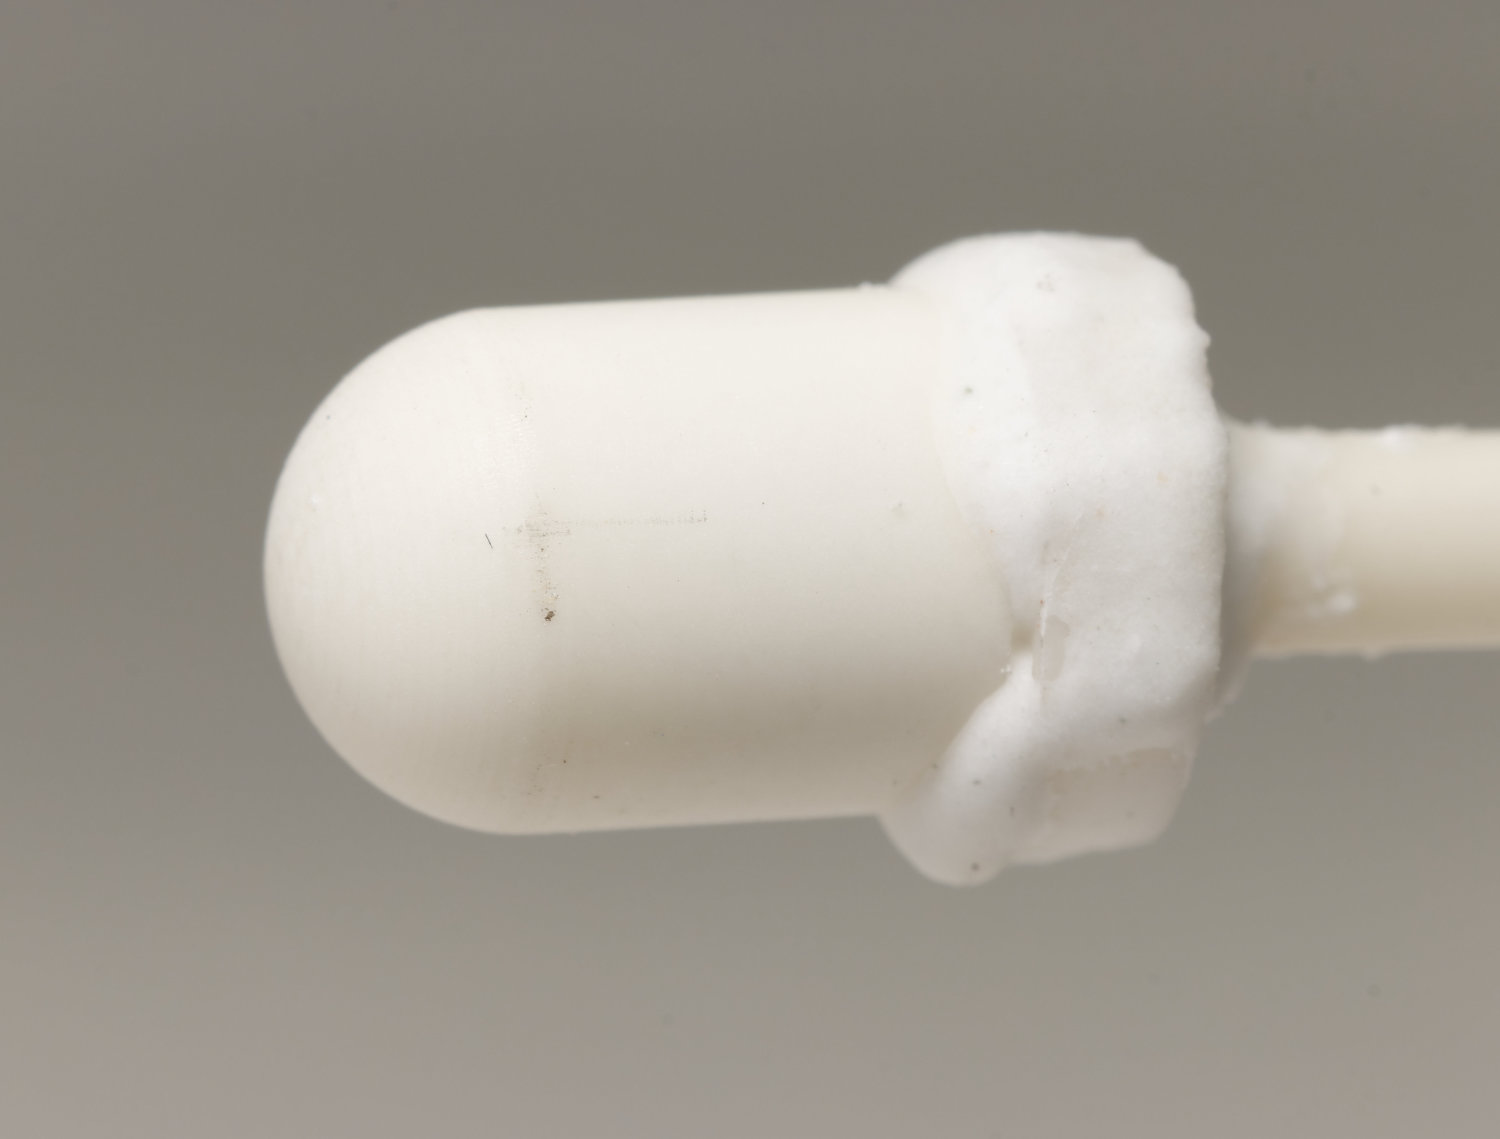
\includegraphics[width=250pt]{figures/bdot_cap.jpg}
	\caption[Ceramic cap of a Bdot probe]{\label{fig:bdot-cap}Ceramic cap of a Bdot probe which is inserted into the LAPD to measure magnetic fluctuations}
\end{figure}

Converting these Bdot signals, after calibration, simply requires integrating $\frac{dB(t))}{dt}$ over time, which is easily accomplished in the frequency domain and avoids accumulating errors. Integrating over $t$ in the frequency domain simply requires dividing by $-i\omega$:

\begin{equation}
	  \int \dot B(t) dt = \int \sum_\omega b_\omega e^{-i \omega t} dt = \sum_\omega \frac{b_\omega}{-i \omega} e^{-i \omega t}
\end{equation}
where $\sum_\omega b_\omega e^{-i \omega t}$ is the Fourier decomposition of $\dot B(t)$

\subsection{The 288 GHz heterodyne interferometer}

The LAPD is equipped with two 288 GHz heterodyne interferometers which measure line-integrated density. These interferometers function by applying a voltage shift to the source of the 288 GHz signal (96 GHz, tripled) using a sawtooth waveform at 750 kHz, leading frequency changes in the range of tens of MHz. Density fluctuations measurable by the interferometer occur much slower than this 750 kHz sweep frequency. When this wave is launched into the LAPD and returned, this 750 KHz wave is phase-shifted relative to a 750 kHz reference caused by both the free-space propagation time and the plasma-induced increased path length. A higher-density plasma leads to an increased path length which leads to a larger observed phase shift. This phase shift can then be unwrapped to obtain a density, given some calibration factor. The reference and detector signals are recorded by an oscilloscope, which can be read from LabView (as part of the MSI system) or python, or written to a file.

\subsection{Thomson scattering}

Thomson scattering is the gold standard of temperature measurements. In the LAPD, the Thomson scattering has been implemented in the non-collective regime using a 532 nm, 460 mJ Nd:YAG laser to measure $T_e$ and $n_e$ \cite{ghazaryan_thomson_2022}. Thomson scattering is the process of electrons scattering and doppler shifting incident light, where the doppler shift is caused by the electron thermal motion. This scattered light is then collected by a spectrometer where the doppler shift is directly measured. The density can also be measured by counting the incident photons after absolute calibration of the entire optical system, including scanning of the fiber coupling optics to maximize signal. Between shots, background spectra are taken and subtracted from the signal to reduce the influence of optical imperfections and spurious light. A notch filter is also used to block reflections from the 532 nm laser.

Analysis is fairly straightforward: the spectrum can be fit assuming a Gaussian distribution if the plasma distribution is Maxwellian. The temperature is determined by the width of the distribution: $T_e = 0.4513 \cdot \Delta \lambda_{1/e}^2$, where $\lambda_{1/e}$ is the half width where the spectrum reduces by $1/e$ \cite{ghazaryan_thomson_2022}. The density can be calculated by integrating this fit distribution, but without a recent and accurate absolute calibration this value is not reliable and should not be used.

The Thomson scattering system benefits from higher density (above $10^{13}$ cm$^{-3}$) and lower temperatures, otherwise many shots (a few thousand) may be required to get a spectrum with a desirable fitting accuracy. Presently, this system measures temperature on-axis at port 32 at a single point in time (span of 4 ns) in the plasma. The measurement volume can be moved to elsewhere in the device with great effort. Coincidentally, a Helium ion line ($7 \rightarrow 4$ transition) at 541 nm is occasionally visible on the spectrum, but the resolution of the spectrometer (0.28 nm) is not sufficient to calculate a thermal doppler shift for reasonable ion temperatures, but it could provide an upper bound.

\subsection{Fast framing camera}

The facility currently has a Phantom v7.3 fast framing camera. At 800 by 600 resolution, it can record at 6,688 frames per second, but can record at over 35,000 frames per second at a 256 by 256 resolution. The camera sensor is 14 bit monochrome and capable of resetting pixels and reacquiring light on event of sensor saturation (the ``extreme dynamic range'' feature). Although this footage is not analyzed in a quantitative way, it is nonetheless useful for building intuition on the structures and dynamics in the device (and worst case, makes for some pretty images). The light collected by the camera has been shown to correlate fairly well with $I_\text{sat}$, at least in the plasma bulk (according to unpublished work by Daniel Guice). 

\section{Instabilities in mirrors and the LAPD}

\subsection{Drift waves}

Drift waves exist in any magnetized plasma that has a density gradient. For this reason, this is often called a ``universal'' wave or instability. 

Pressure gradient in a slab
Any resistivity leads to charge separation and instability growth
Show diagram 

\subsection{Rotational interchange}



\subsection{Interchange}

Pressure gradient aligned with curvature vector
Showstopper for earlier mirror machines

\section{Machine learning and neural networks}

Fundamentally, neural networks (NNs) are a function that, given sufficient capacity, can represent any function -- this is the ``universal approximation theorem''. Stated succinctly, NNs are fancy curve fits. As we will see in this work, fancy curve fits can be very useful.

\subsection{Fundamentals of neural networks}

Neural networks are built one `layer' at a time. A layer in an NN is a vector $\vec x_i$ multiplied by some weight matrix $\mathbf{W}$ followed by a nonlinearity to get the activation $x_{i+1}$:
\begin{equation}
	\vec x_{i+1} = f( \mathbf{W} \vec x_i)
\end{equation}
where $\vec x_i$ is the previous activation (or input). A bias $b$ (a learnable offset) is often concatenated to the input vector beforehand. The activation function $f$ can be any nonlinearity. Typical choices for $f$ include the rectified  linear unit -- ReLU (zero when the input is less than zero, linear otherwise), tanh, sigmoids, sigmoid linear unit (SiLU), and so on. ReLU, and a variant of which called Leaky ReLU, are popular choices given the simplicity of computation.

Stacking these layers one after another leads to the ability to express very complex curves. The true innovation here is the ability to express very high dimensional curves which was otherwise impossible until the advent of modern NN techniques, enabled by fast matrix multiplication hardware (read: GPUs).

The weights of these layers are trained via gradient descent of some loss function $\mathcal{L}$. The loss is effectively the penalty for the network predicting the incorrect answer. A typical loss function for regression tasks is the mean-squared error: 
\begin{equation}
	\mathcal{L} = \frac{1}{M} \sum_{i=1}^M (x_i - g(x_i))^2
\end{equation}
where $g(x)$ is the output of the neural network and $x_i$ is a training example in a batch size M. Training over a dataset is often done in batches to reduce the memory required and to introduce stochasticity into the training process which can improve generalization. 

Gradient descent is the process of modifying the NN weights by calculating the gradient of the loss function with respect to those weights:
\begin{equation}
	\theta \gets \theta - \nabla_\theta \mathcal{L}
\end{equation}
Advanced purpose-built algorithms exist to do this gradient descent in a fast manner, the most popular being Adaptive Moment Estimation, known as Adam  \cite{kingma_adam_2017}. 


\subsection{Common layer types}

In this work we use three types of NN layers. First is the dense layer, also referred to as a ``fully-connected'' layers or ``multilayer perceptron'' if the entire model uses dense layers. In this layer every input is connected to every output. This fully-connected topology can lead to very large parameter counts if these layers are repeatedly stacked with a large width.

Second: the convolutional layer, or convolutional neural network (CNN) \cite{lecun_convolutional_1995}. Technically a misnomer (it should be a ``correlation''), this layer scans along the input with a smaller NN. The input dimension of this layer is the ``kernel size'', and the different networks scanning across the input are the ``filters''. These CNNs have been used to great effect in image processing and time series analysis and are relatively parameter-efficient.

Third: the attention layers. These layers have three inputs called the query, key, and value. When these are all the same the mechanism is called ``self-attention''. The query and key are matrix-multiplied and converted to a probability distribution via a softmax function. This softmax result is then applied to the value. The result of this combination is mask that selects important parts of the value vector. Stacking many of these layers, with multiple self-attention mechanisms for the same input vectors, creates a ``transformer'' \cite{vaswani_attention_2017} which is the basis for the recent advancements in large language models. Here we use these attention mechanisms more modestly.


